\documentclass[12pt,a4paper]{article}

\usepackage[margin=1in]{geometry}
\usepackage{fancyhdr}
\usepackage{graphicx}
\usepackage{epsfig}
\usepackage{parskip}
\usepackage[ansinew]{inputenc}
\usepackage{amsmath}
\usepackage{amssymb}
\usepackage{bm}
\usepackage{float}
\usepackage[free-standing-units=true]{siunitx} % for consistent handling of SI units
\usepackage[colorlinks=true, pdfstartview=FitV, linkcolor=blue, citecolor=blue, urlcolor=blue]{hyperref} % enable links

\setlength{\parindent}{0pt}

\newcommand{\m}[1]
{\mathrm{#1}}

\title{Experiment 83: Do-it-yourself Spectrometer}
\author{Noa Sendlhofer, Christian Leser}
\date{\today}

\begin{document}

\maketitle

\begin{abstract}
    The goal of this experiment series is to determine the temperature of absolute zero, 
    as well as the temperature of liquid nitrogen. An apparatus of constant volume is filled with a gas
    and connected to a pressure sensor. Changing temperatures result in changes in pressure inside the chamber.
    Influences like the pressure and temperature inside the lab, as well as the expansion of the chamber itself
    in changing temperatures must be considered when discussing the obtained data. We concluded that the temperature
    of absolute zero $t_0 = (-275.9 \pm 2.45)\si{\bf\celsius}$ and the temperature of liquid nitrogen $t_{LN2} = (-198.5 \pm 2.56)\si{\bf\celsius}$.
    The literature values lie within our error margins.

\end{abstract}

\tableofcontents

\section{Introduction}

    % Interference double-silt source: https://wiki.anton-paar.com/ch-de/doppelspaltexperiment/
    % Interference grating source: https://www.grund-wissen.de/physik/optik/wellenoptik.html
    % Grating constant source: https://ieeexplore.ieee.org/stamp/stamp.jsp?tp=&arnumber=5547333&tag=1 (eth network)
    % Lands Pits CD source: https://www.researchgate.net/figure/Lands-and-pits-image-using-a-scanning-electron-microscope_fig3_221291847
    

    The goal of this experiment series is to build a spectrometer using household objects by making use of the wave character of light.
    To understand how the spectrometer works, we need to take a close look at how light behaves under certain conditions.

    \begin{figure}[H]
        \centering
        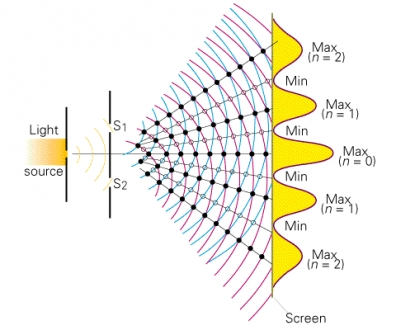
\includegraphics[scale = 0.7]{src/images/interference_double_slit.jpg}
        \caption{Double slit experiment.
        The interference of the light waves produce aspecific pattern which depends of the wavelength of the light entering the slits as well as the distance between the slits. \cite{src_double_slit}}
        \label{fig_double_slit}
    \end{figure}

    Light travels in a spherical way behind a slit meaning that each slit acts as a new source of waves.
    These waves interfere with each other as they overlap, resulting in an interference pattern of alternating bright and dark regions on the screen or detector.
    This behaviour is due to the fact that two maxima or minima intensify each other while a maximum and a minimum cancel out.
    We also refer to these two cases as constructive and destructive.
    Figure~\ref{fig_double_slit} shows how this effect works.

    \begin{minipage}{0.99\linewidth}
        \begin{minipage}{0.7\linewidth}
            \begin{figure}[H]
                \centering
                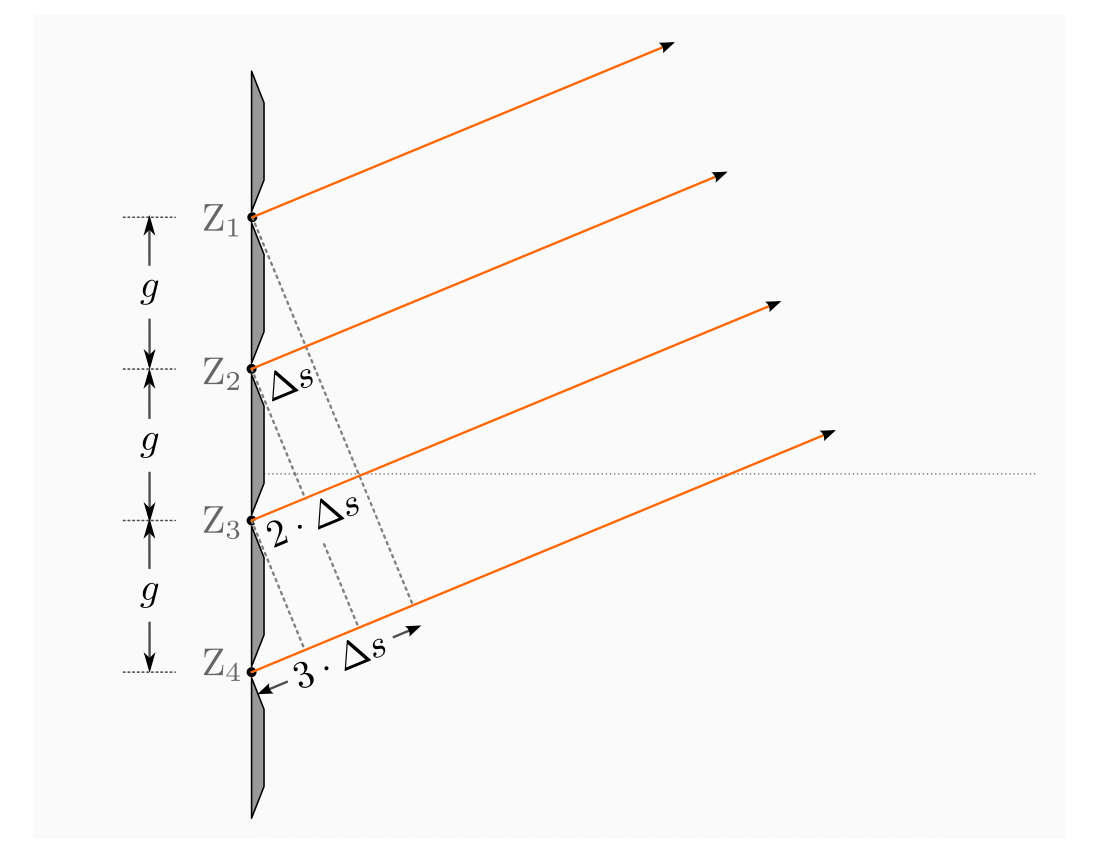
\includegraphics[scale = 0.25]{src/images/interference_grating.png}
                \caption{A grating leads to a similar effect as a double slit.
                $\Delta s$ is equal to the wavelength.
                As seen in the figure, the angle at which brighter spots of light can be seen depends on the wavelength. \cite{src_grating}}
                \label{fig_grating}
            \end{figure}
        \end{minipage}
        \begin{minipage}{0.25\linewidth}
          \begin{scriptsize}
            \begin{center}
                \begin{figure}[H]
                    \centering
                    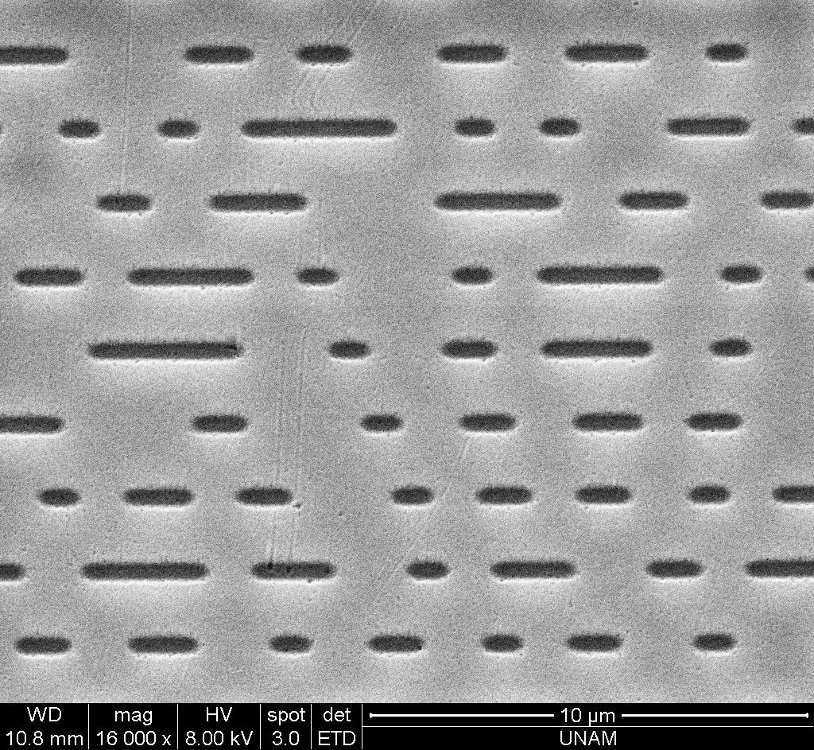
\includegraphics[scale = 0.15]{src/images/lands_pits_cd.png}
                    \caption{Lands and pits image of a CD using a scanning electron microscope. These form a grating too. \cite{src_cd}}
                    \label{fig_lands_pits}
                \end{figure}
            \end{center}
            \end{scriptsize}
        \end{minipage}
    \end{minipage}

    Moving on to a grating, it can be abstracted as a lot of slits next to each other.
    Hence, the effect is almost the same as the one observed at the double slit.
    Most importantly, an interference pattern can be observed too.
    When taking a close look at a CD, we notice a grating, presented in figure~\ref{fig_lands_pits}.
    In consequence, a CD must also produce an interference pattern in which light of different wavelength can be observed and distinguished.
    The characterisation of the light is done by measuring the distance of the maximum of first order as it is dependent of the wavelength.

    \begin{minipage}{0.99\linewidth}
        \begin{minipage}{0.45\linewidth}
            \begin{figure}[H]
                \centering
                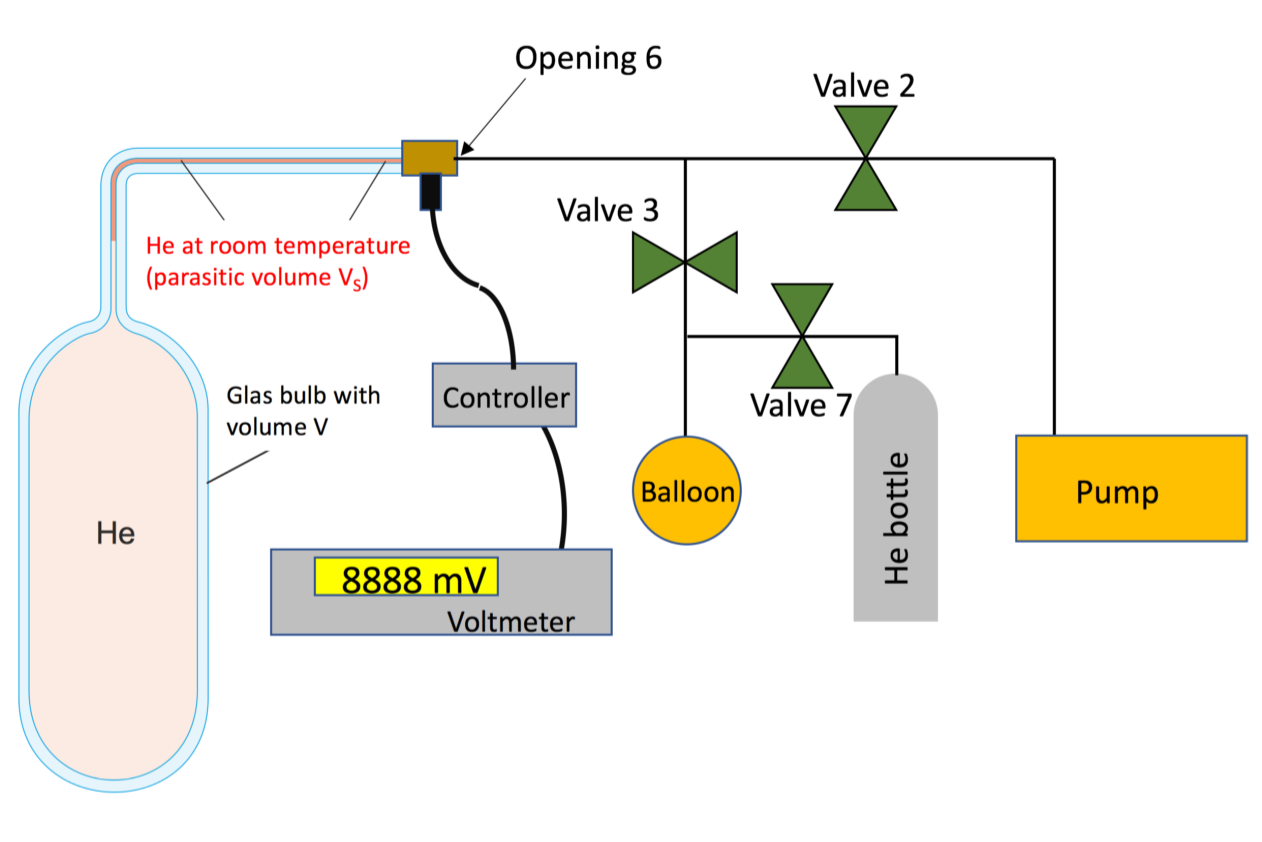
\includegraphics[scale = 0.4]{src/images/experimental_setup.png}
                \caption{Schematic of the experimental setup.
                A source emits rays of light of which a small portion enters the apparatus through a gap between two razor blades of about 0.2 mm.
                the light then travels through the dark chamber, until it hits the CD.
                After passing through the grid on the CD, an interference pattern can be detected using a camera.}
                \label{fig_setup}
            \end{figure}
        \end{minipage}
        \begin{minipage}{0.1\linewidth}
        \end{minipage}
        \begin{minipage}{0.45\linewidth}
          \begin{scriptsize}
            \begin{center}
                \begin{figure}[H]
                    \centering
                    \includegraphics[scale = 0.05]{src/images/spectrometer.png}
                    \caption{Experimental setup used in our case.
                    A phone is used as the camera to detect the interference pattern.}
                    \label{fig_spectrometer}
                \end{figure}
            \end{center}
            \end{scriptsize}
        \end{minipage}
      \end{minipage}
    


    % In general this section should tell the reader why he or she should
    % be interested in your paper. Give some background to the
    % experiment, and describe the underlying principles. This is typically where you provide references to previous publications~\cite{Sato2003}. % Christian

\section{Methodology}~\label{sec_methodology}
    % Über Bau des Spektrometers erzählen
    % Formeln erklären
    % Argumentieren warum wir grating constant vom internet nehmen

    To build the spectrometer, cardboard, tape, two razor blades, a CD and a camera (ideally wide angle) are needed.
    The less reflective the cardboard is, the better the results are going to be.
    Build a tube with the cardboard and attach the two razor blades to one end, leaving just a small slit of about 0.2 mm for light to enter.
    Remove the reflective foil off the CD using a cutter and tape and cut out a piece of the transparent part of the size of the cardboard tube.
    tape it to the open end of the tube.
    Now attach the camera to the same side.
    make sure no light enters the apparatus except through the slit.

    If held in the direction of a light source, a diffraction pattern, showing the spectrum of the different wavelengths, is visible on the camera.
    The formula relating the distance of the maxima of different orders to the wavelength of the light entering the spectrometer is given in equation~\eqref{eq_interference}.
    \begin{align}
        p \lambda = g \sin(\phi) \label{eq_interference}
    \end{align}

    $p$ is an integer called the order number. For the first visible maximum, $p$ is equal to $1$, for the second maximum $p = 2$ and so on.
    $\lambda$ is the wavelength of the light.
    The grating constant $g$ is dependent on the distance between the slits in the grating.
    Hence this constant is not the same for different kinds of CDs or DVDs.
    the last variable is the angle $\phi$ in the triangle of the maximum of zero and $p^{th}$ order and the spot where the light passes through the grating, measured at the grating.
    Trigonometry gives the relation in equation~\eqref{eq_phi}, which is visible in the figure~\ref{fig_phi}.
    \begin{align}
        \tan(\phi) = \frac{x_p}{d} \label{eq_phi}
    \end{align}

    \begin{figure}[H]
        \centering
        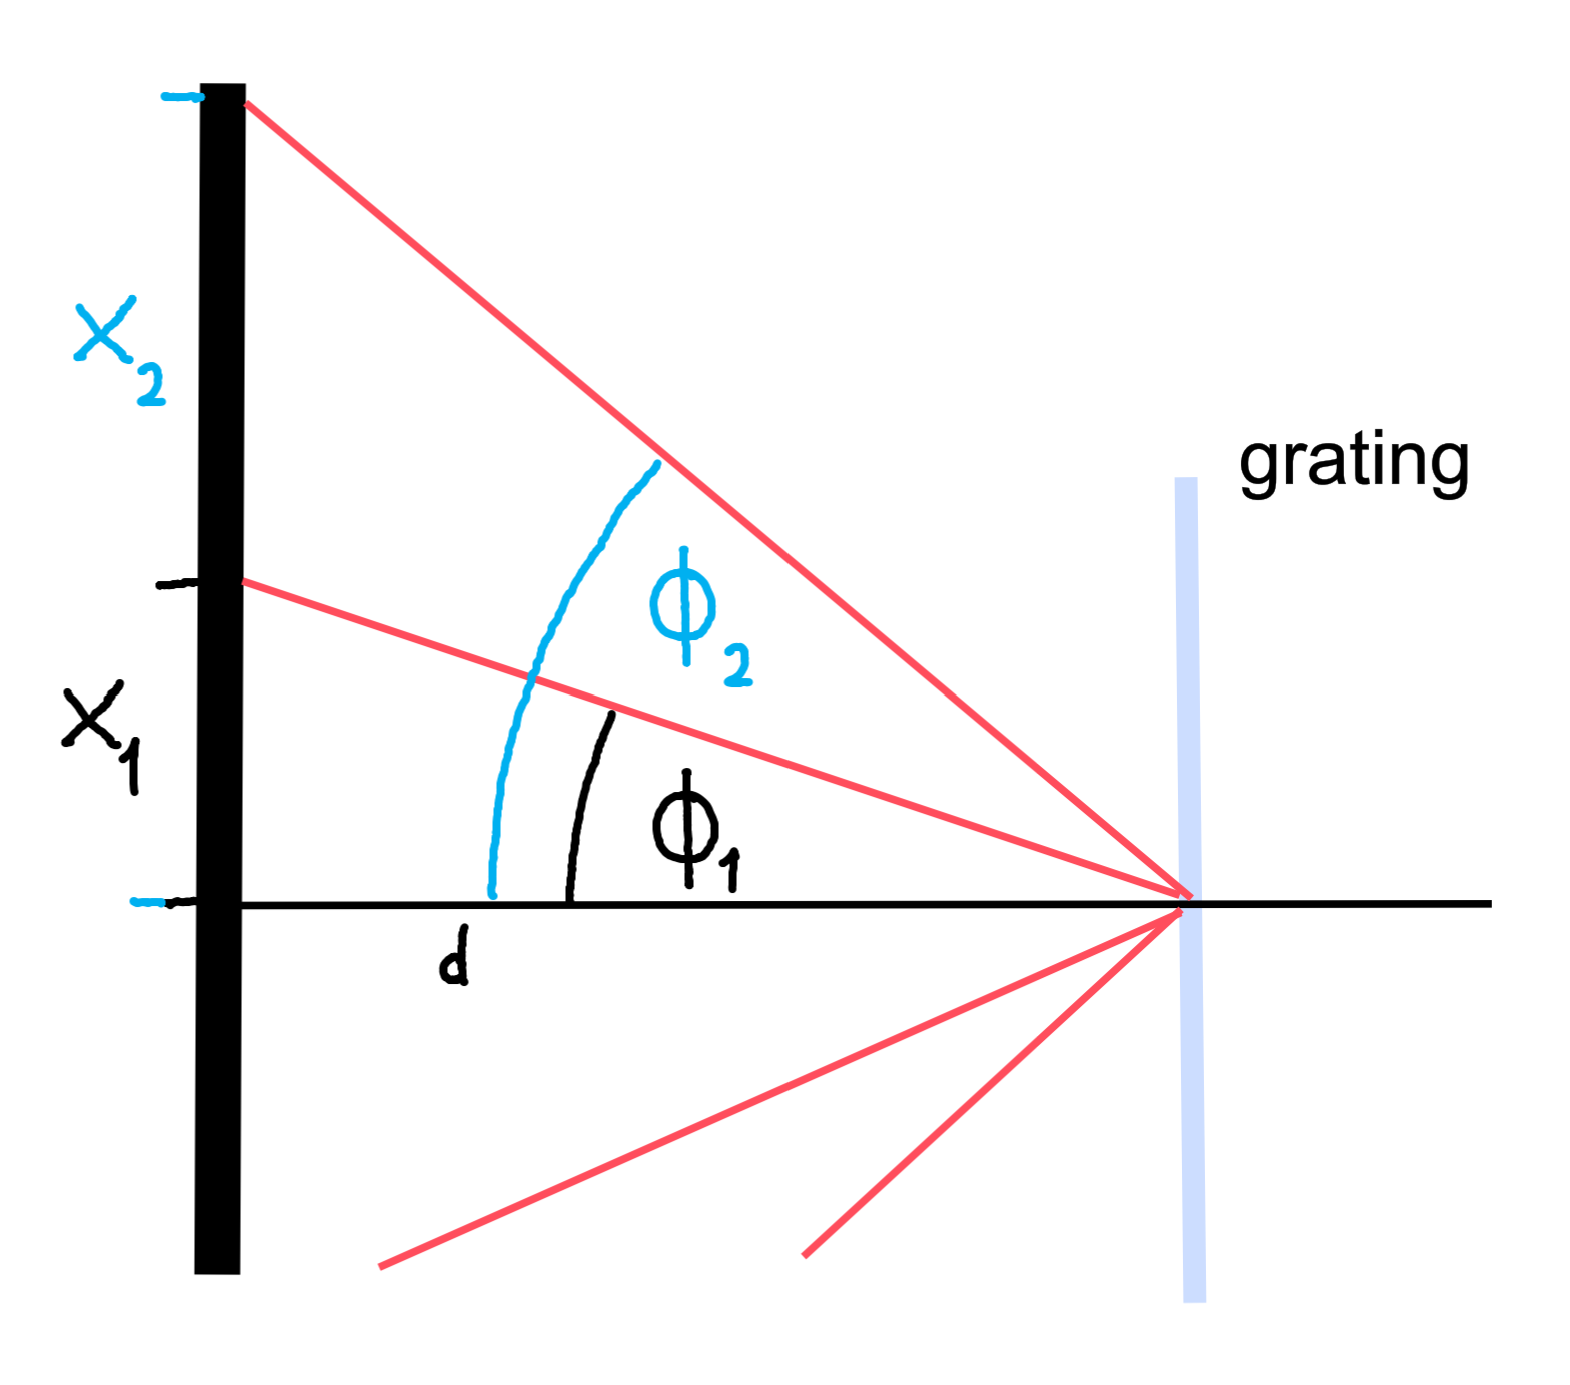
\includegraphics[scale = 0.6]{src/images/angle_phi.png}
        \caption{Visualization of the location of the angle $\phi$ referred to in equation~\eqref{eq_interference}.
        The first and second maximum of one certain wavelength is shown, so monochromatic light would be needed to reproduce this hypothetical situation.}~\label{fig_phi}
    \end{figure}

    In our test case, we assumed a grating constant $g = 1.514 \mu m$~\cite{src_grating_constant} as we did not have a monochromatic light source at hand to determine the grating constant of our CD.\@
    Monochromatic light ensures that the interference pattern produced by the grating is sharp and well-defined, while polychromatic light sources show a transition in colors.
    Hence, polychromatic light sources are a lot less precise for calibration.
    Next, we calculated the distance between the CD and the camera to calibrate our spectrometer using a first measurement and by choosing a certain color and its corresponding wavelength by eye.

    Now, having a calibrated and working spectrometer, we did multiple measurements of different light sources.

    With a good spectrometer, it is possible to observe dark lines in the spectrum of sunlight, known as Fraunhofer lines.
    They result from the absorption of specific wavelengths of light by the outer layers of the Sun, giving information about the composition of gases in the atmosphere.

    \subsection{Different types of light sources}

    The most common natural light sources are stars and fire. The first process happens due to fusion reactions, while the
    second is a chemical reaction.

    Artificial light sources can be roughly categorized into the following groups:

    Traditional Bulbs:
        Traditional light bulbs generate light by passing electricity through a certain metal wire, which causes it
        to heat up to a point where it produces light.

    Discharge Lamps:
        Discharge lamps produce light through the process of electric discharge in a gas or vapor 
        contained within the lamp. There are different variations of this process depending on the exact
        type of lamp used.

    Light-emitting diodes (LED) are semiconductors that produce light through electroluminescence.
    This method is very energy efficient, which is why they are widely used today.

    In our experiment, we were able to analyze LED lighting, sunlight, as well as a fluorescent tube, which is a type of discharge lamp.

\newpage

\section{Results}\label{sec_results}

\subsection{Calculation of the grating constant $g$}

In our case, we will calculate the grating constant $g$ using hypothetical values for the reasons mentioned in section~\ref{sec_methodology}.
By rearranging and combining eq.\ref{eq_interference} and eq.\ref{eq_phi} we find a formula for the grating constant\ref{eq_g}.

\begin{align}
    g &= \frac{p \lambda}{\sin(\phi)} \label{eq_g}\\
    \phi &= \arctan \left( \frac{x}{D} \right)
\end{align}

To calculate the uncertainty of the grating constant, the gaussian error propagation was used.
\begin{align}
    \Delta g &= \sqrt{\left( \frac{\partial g}{\partial p} \Delta p \right)^2 + \left( \frac{\partial g}{\partial \lambda} \Delta \lambda \right)^2 + \left( \frac{\partial g}{\partial \phi} \Delta \phi \right)^2}\\
    \Delta \phi &= \sqrt{\left( \frac{\partial \phi}{\partial x} \Delta x \right)^2 + \left( \frac{\partial \phi}{\partial D} \Delta D \right)^2}
\end{align}

The hypothetical value of the grating constant $g$ and its uncertainty can now be calculated:
\begin{align}
    \bf g = (1520 \pm 20) ~\si{\bf\nano\meter} = (1.52 \pm 0.02) ~\si{\bf\micro\meter} \label{res_g}
\end{align}

Note that the obtained value is not the real value and that a different value for the grating constant $g$ \cite{src_grating_constant} is used in the remaining calculations.

\subsection{Calculation of the distance $d$}

As mentioned in the previous chapter, the first goal is to find the distance $d$ of the grating
and the image sensor.
By combining eq. \ref{eq_interference} and eq. \ref{eq_phi} we get the following equation for $d$:
\begin{align}
    d = \frac{x}{\tan(\phi)} = \frac{x}{\tan(\arcsin(\frac{\lambda}{g}))} \label{eq_distance}
\end{align}

Multiple steps are necessary to calculate the distance $d$.
First of all, we took a picture with the spectrometer pointed at the sunlight (fig.~\ref{fig_sunlight}). We then selected suitable 
points in the spectrum and compared them to tabulated wavelengths and their corresponding colors 
in fig.~\ref{fig_wavelengths}. In the next step we measured the distance $x$ required in eq.~\ref{eq_distance} of said points to the zero-order maximum
using the imtools method in matlab.

For our final calculation of the distance $d$ we averaged multiple measurement points to get a more
accurate result. This is shown in fig.~\ref{fig_sunlight}.

The error calculations for eq. \ref{eq_distance} were done using the gaussian error propagation.
Please refer to our jupyter notebook \cite{GitHub}, for the full calculations of all the values and 
error propagations presented in this chapter. 
\begin{align}
    \Delta d = \sqrt{\left(\frac{\partial d}{\partial x}\right)^2 + \left(\frac{\partial d}{\partial \lambda}\right)^2}
\end{align}

Our average result for the distance $d$ is:
\begin{align}
    \bf d = (1.7 \pm 0.1) ~\si{\bf\milli\meter} \label{res_d}
\end{align}

We have now successfully calibrated our spectrometer and we can now determine the wavelength
of any point in the picture.
The following equation is used to determine the wavelength of a point with a certain pixel 
distance $x$ to the zero-order maximum.
\begin{align}
    \lambda = g \sin\left(\arctan\left(\frac{x}{d}\right)\right) \label{eq_lambda}
\end{align}

Again the uncertainties were determined using the gaussian error propagation.
\begin{align}
    \Delta \lambda = \sqrt{\left(\frac{\partial \lambda}{\partial x}\right)^2 + \left(\frac{\partial \lambda}{\partial d}\right)^2}
\end{align}

\subsection{Analysis of different light sources}

Using these obtained results we finally analyzed some different types of light sources. In each case, we assumed 
an error of $\pm 10$ pixels, since we had to choose the position of each measurement point in the picture by hand.

First of all, we analyzed a fluorescent tube lamp. As can be seen in fig. \ref{fig_lamp1} below, this type of 
light source only emits certain small ranges of wavelength. In our case, we measured the following ranges:
\begin{alignat}{3}
    &\text{Red spectrum:} \; &&(587 \pm 36)~\si{\nano\meter} & &- (622 \pm 38)~\si{\nano\meter} \nonumber\\
    &\text{Green spectrum:} \; &&(487 \pm 32)~\si{\nano\meter} & &- (560 \pm 35)~\si{\nano\meter} \nonumber\\
    &\text{Blue spectrum:} \; &&(430 \pm 29)~\si{\nano\meter} & &- (455 \pm 31)~\si{\nano\meter} \nonumber
\end{alignat}
\vspace{-2em}
\begin{figure}[H]
    \centering
    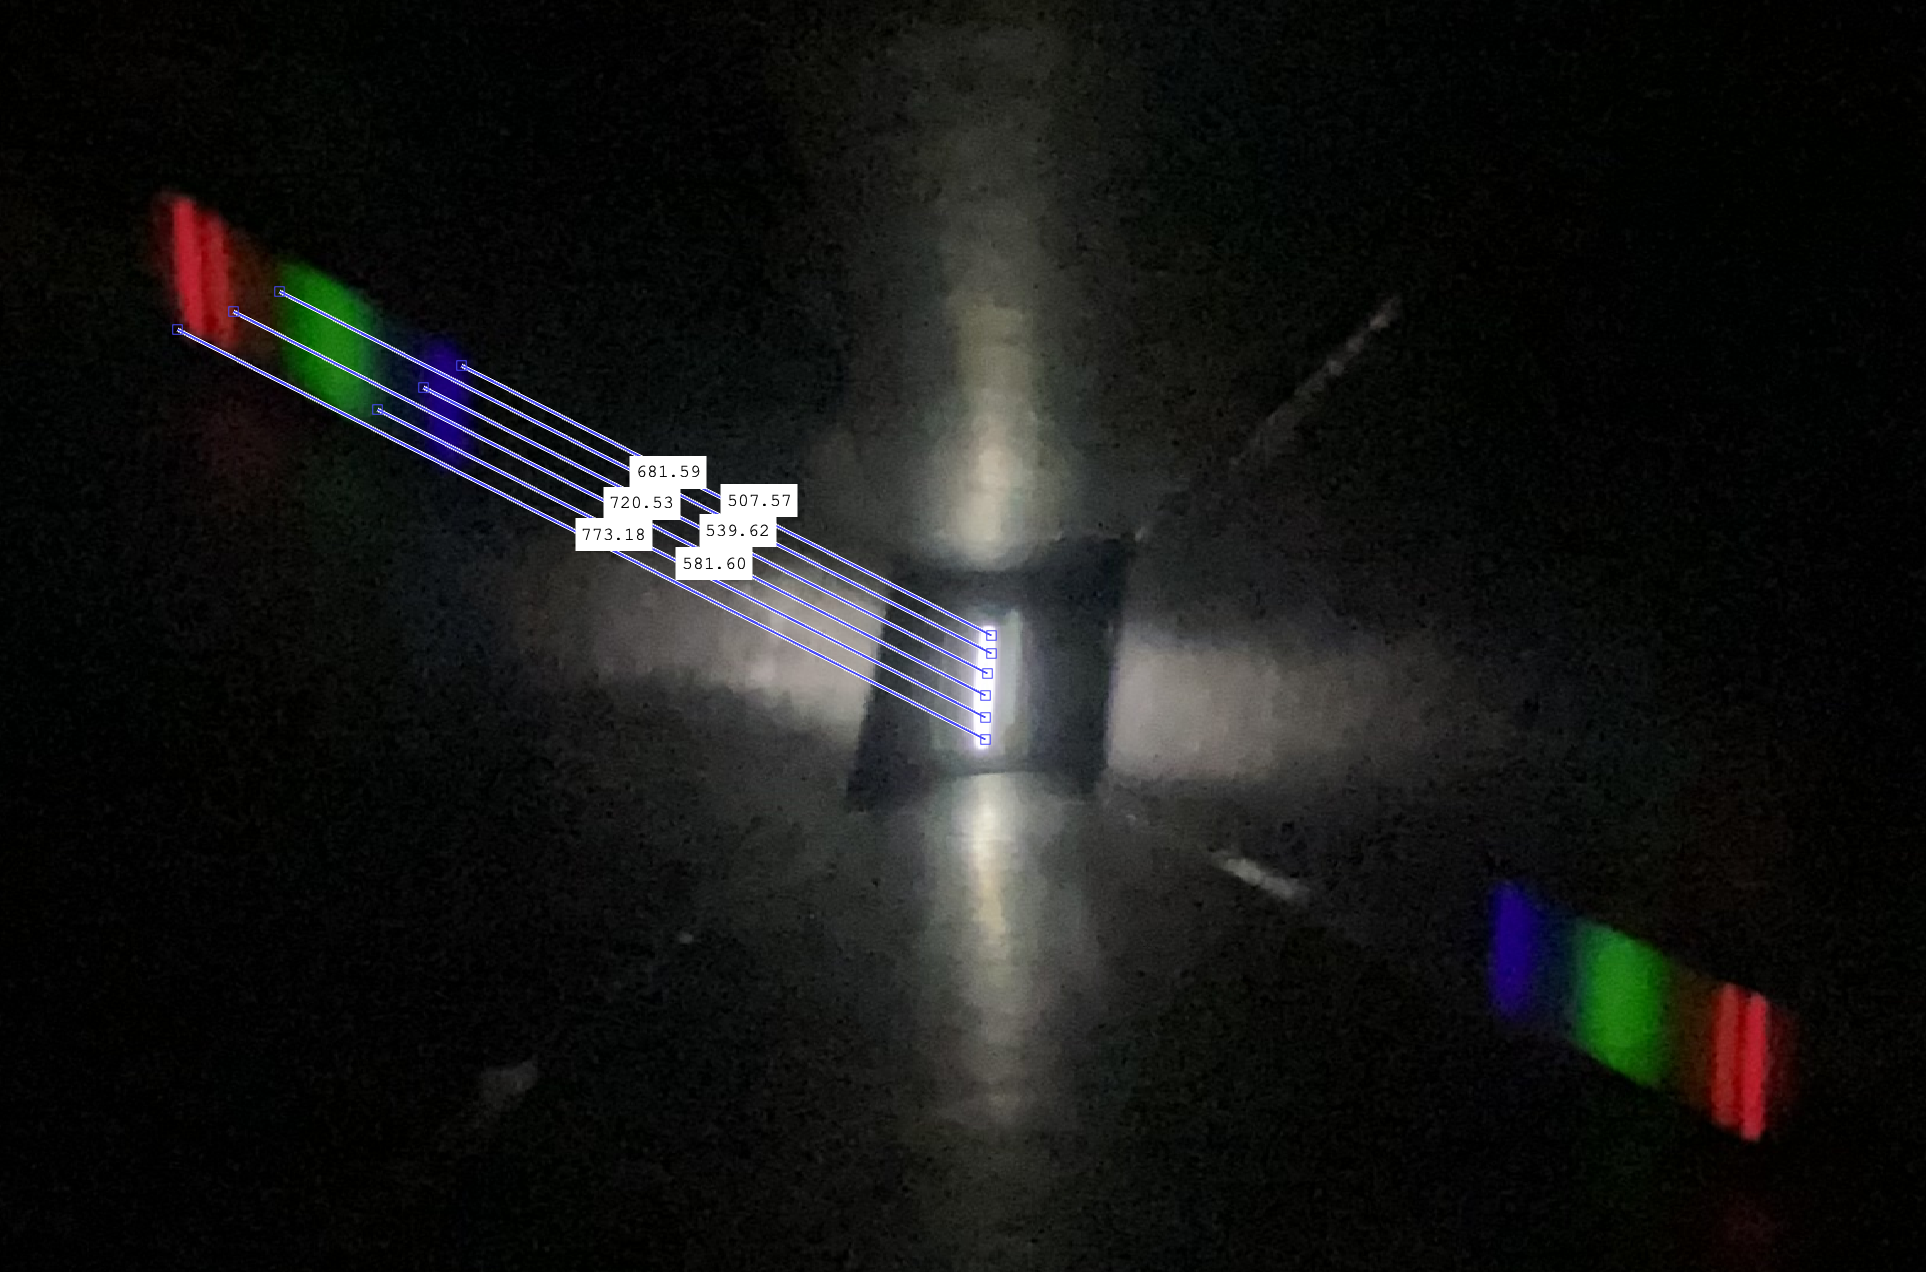
\includegraphics[scale = 0.28]{src/images/lamp1_meas.png}
    \caption{Spectrum of a fluorescent tube.}
    \label{fig_lamp1}
\end{figure}

As a second example, we analyzed a LED ceiling lamp. As can be seen in fig. \ref{fig_lamp2} below, this lamp
emits almost the entire spectrum of visible light with no gaps visible. We measured the following range:
\begin{alignat}{3}
    &\text{Full spectrum:} \; &&(429 \pm 29)~\si{\nano\meter} & &- (650 \pm 38)~\si{\nano\meter} \nonumber
\end{alignat}
\vspace{-2em}
\begin{figure}[H]
    \centering
    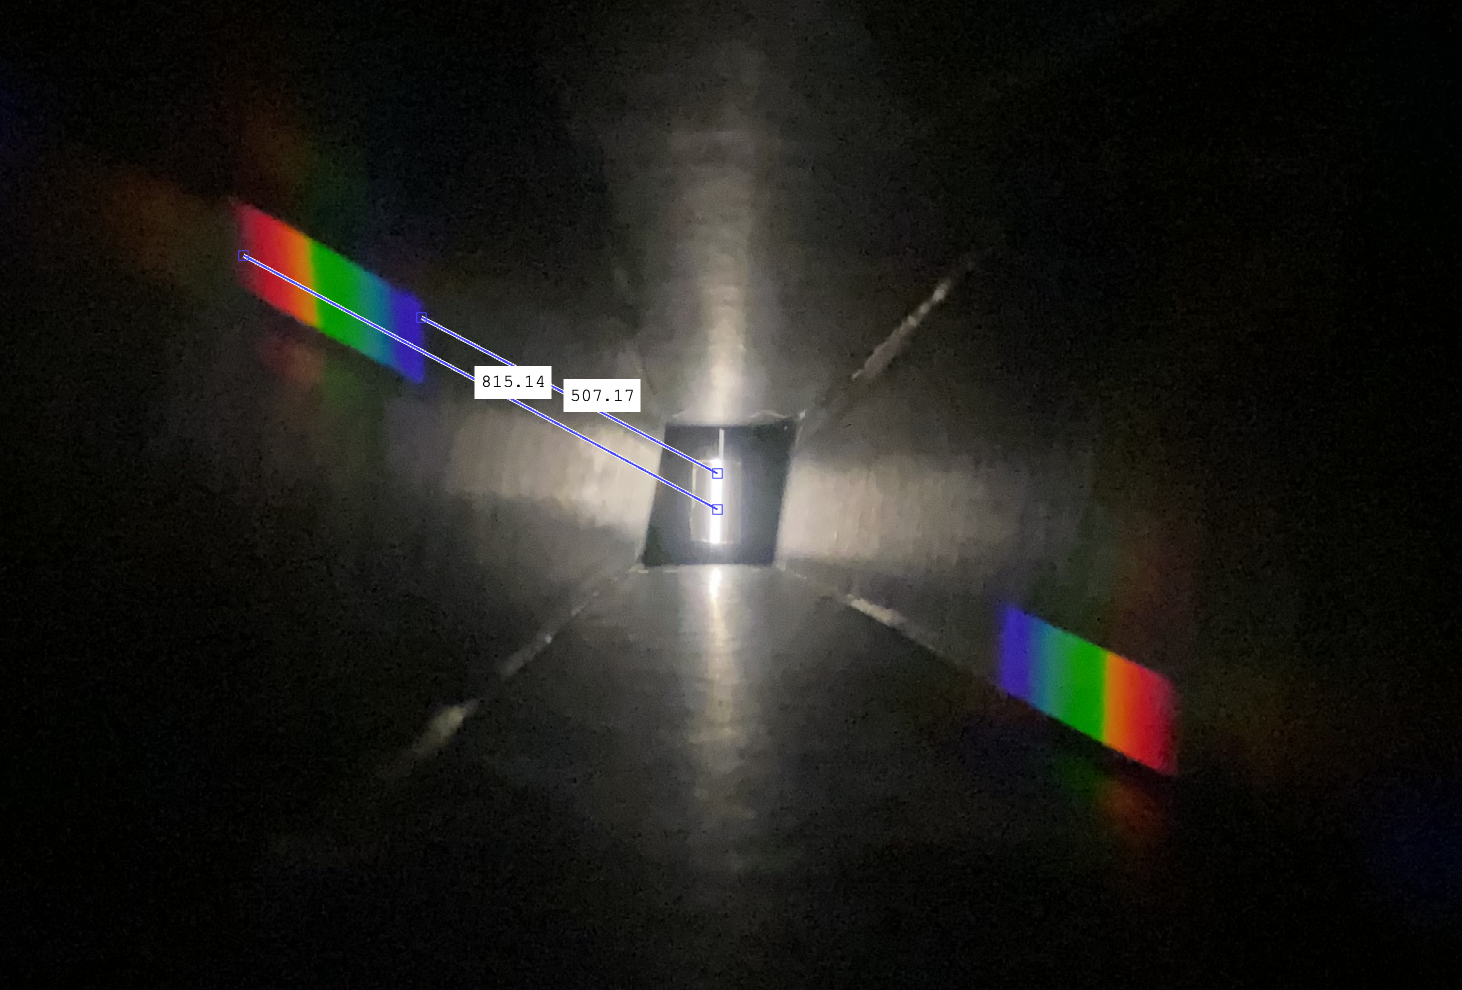
\includegraphics[scale = 0.38]{src/images/lamp2_meas.png}
    \caption{Spectrum of an LED ceiling light.}
    \label{fig_lamp2}
\end{figure}

Lastly, we analyzed the computer screen of a laptop. In this example, the color purple was shown on the screen.
As can be seen in fig. \ref{fig_purple_screen} only two very narrow bands of wavelengths are emitted.
\begin{alignat}{3}
    &\text{Red spectrum:} \; &&(597 \pm 37)~\si{\nano\meter} & &- (622 \pm 38)~\si{\nano\meter} \nonumber\\
    &\text{Blue spectrum:} \; &&(433 \pm 29)~\si{\nano\meter} & &- (457 \pm 37)~\si{\nano\meter} \nonumber
\end{alignat}
\begin{figure}[H]
    \centering
    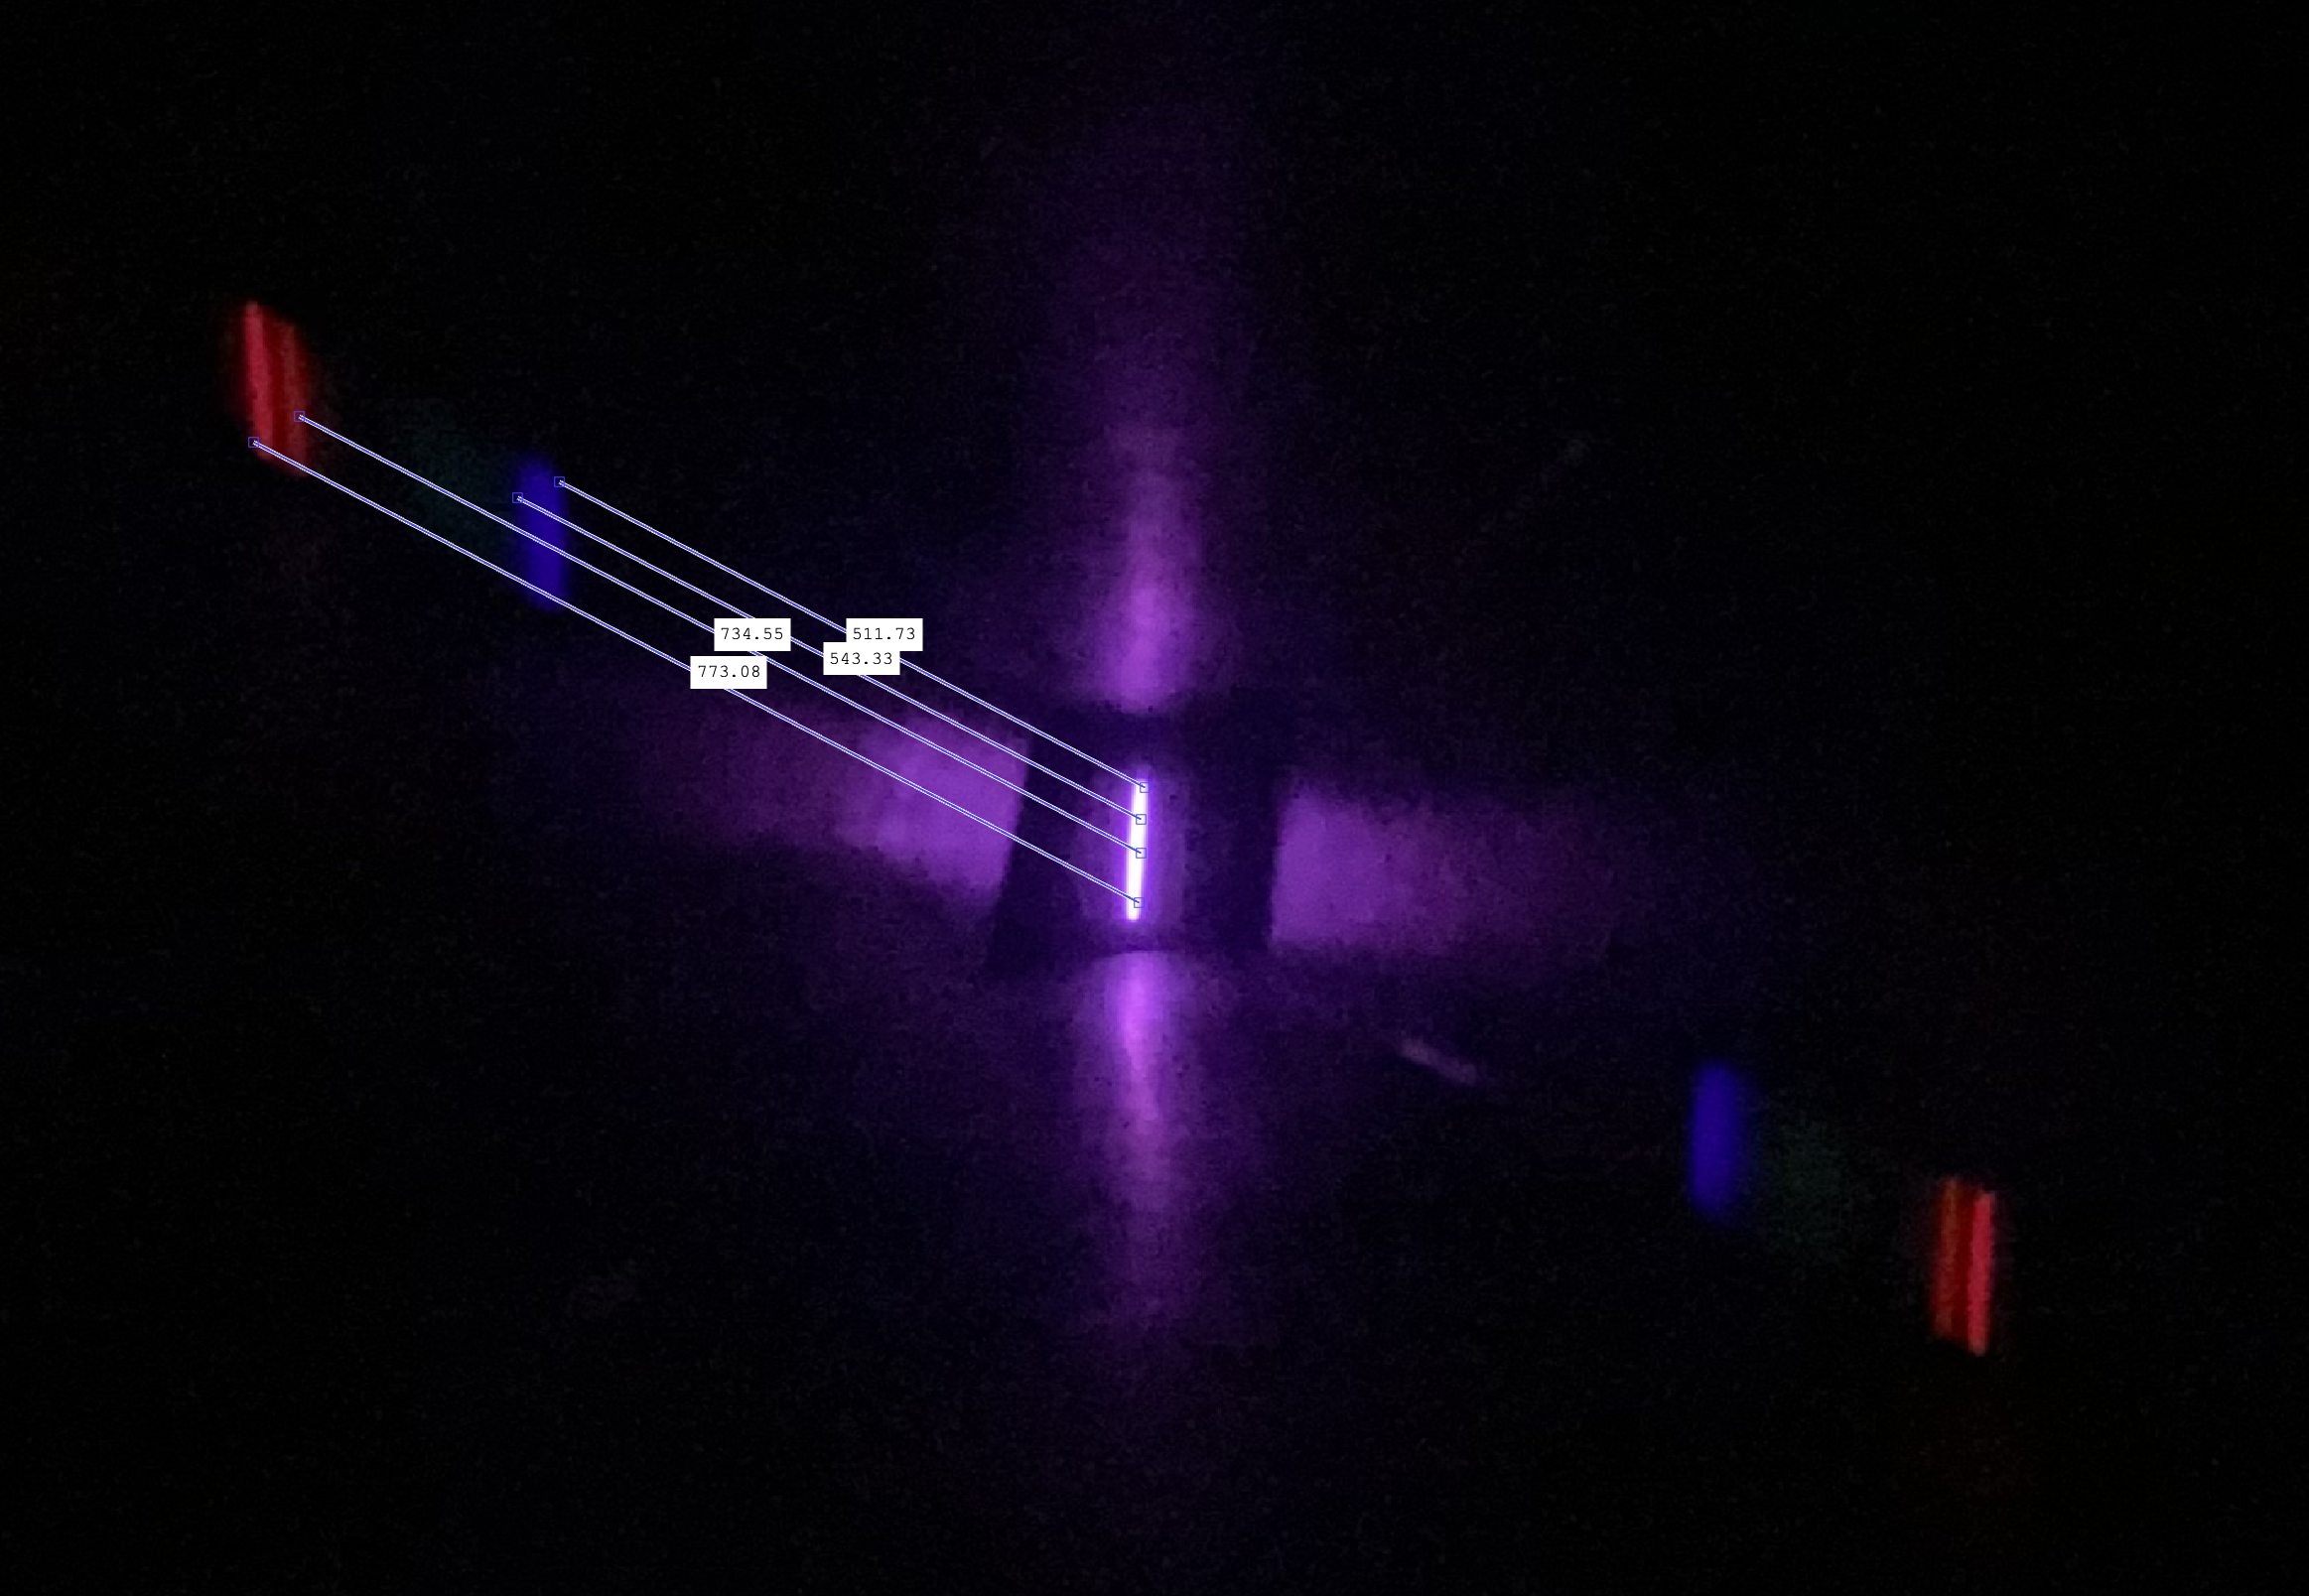
\includegraphics[scale = 0.24]{src/images/purple_screen_meas.png}
    \caption{Spectrum of a computer screen displaying a purple color.}
    \label{fig_purple_screen}
\end{figure}

Modern computer screen use LEDs as a light source. Typically the screen consists of many small red, blue and 
green LEDs that are located next to each other in a repeating pattern. Even though only a small fraction of 
the entire visible spectrum of light is emitted these screens can reach a very high color accuracy. Our eyes 
contain three different types of receptors, that can detected different ranges of wavelengths corresponding 
to the colors red, green and blue. Our brain generates a color by mixing the information of these receptors, 
which is why the color on our screens seem natural to us.

\subsection{Theoretical spectra of light sources}

In the experiment 15 two different light sources were analyzed: A helium discharge tube, as well as
a mercury light. These are not commonly available types of light sources. Both lamps only emit very narrow bands
of wavelengths. We took the expected wavelength values from literature, as cited below.

In the following figure~\ref{fig_helium_spectrum}, the expected wavelengths of a helium discharge tube are 
drawn into the spectrum of sunlight. \cite{Helium Discharge Tube}
\begin{figure}[H]
    \centering
    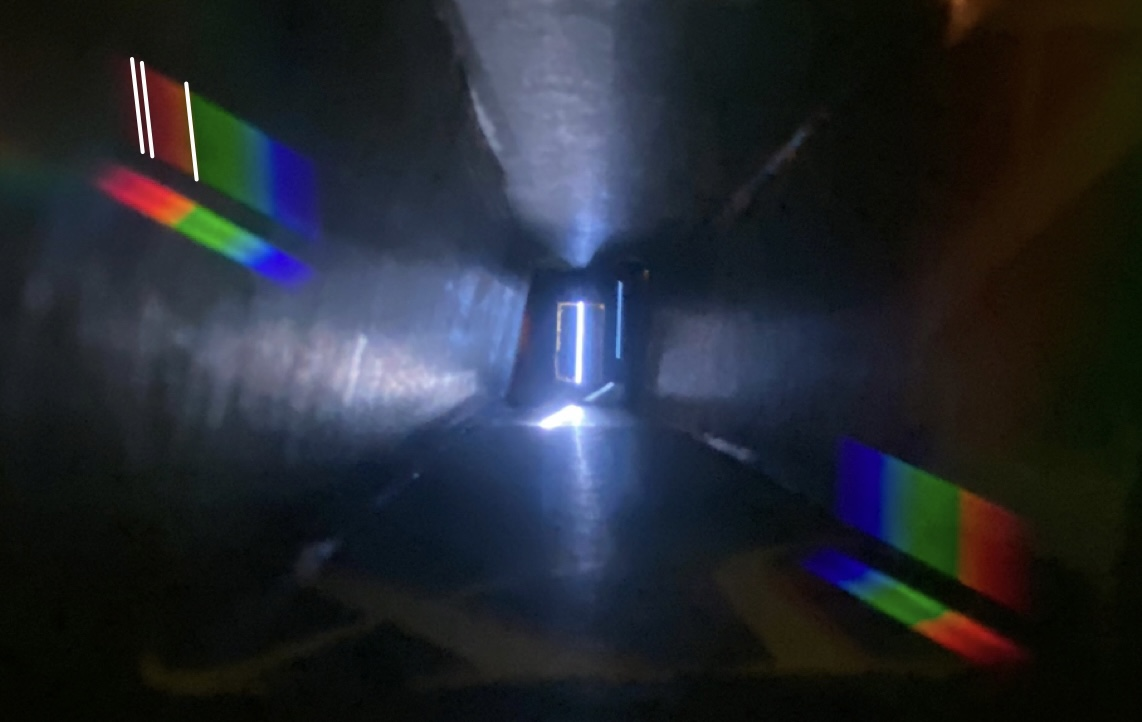
\includegraphics[scale = 0.23]{src/images/helium_spectrum.jpg}
    \caption{Expected helium spectrum is drawn in white color into the spectrum of sunlight.}
    \label{fig_helium_spectrum}
\end{figure}
\vspace{-1em}
Lastly in the following figure, the expected wavelengths of a mercury light are drawn into the spectrum of sunlight.
\cite{Mercury Vapor Lamp}
\begin{figure}[H]
    \centering
    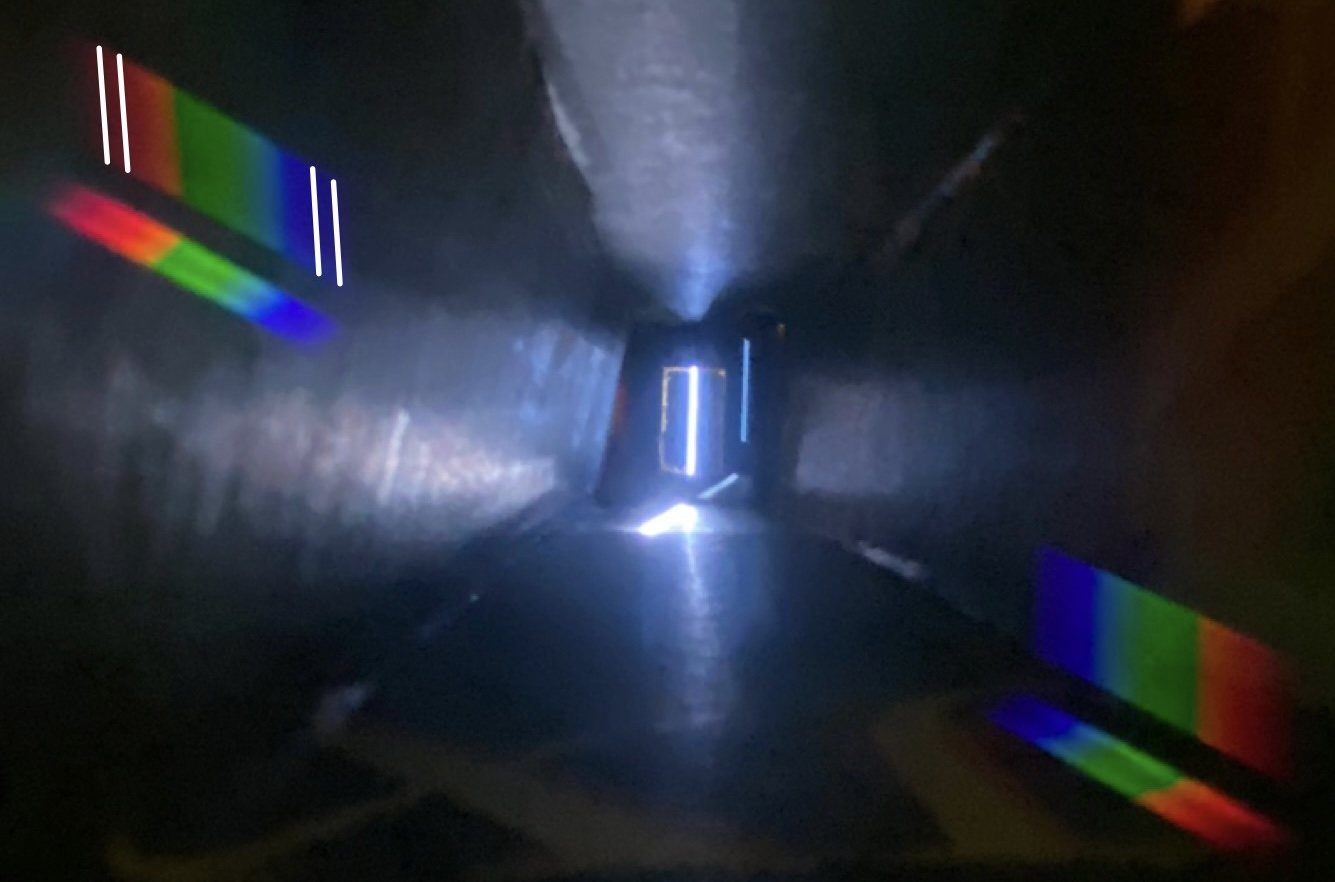
\includegraphics[scale = 0.2]{src/images/mercury_spectrum.jpg}
    \caption{Expected mercury spectrum is drawn in white color into the spectrum of sunlight.}
    \label{fig_mercury_spectrum}
\end{figure} % Noa Results

\section{Conclusion}
    In this experiment series, we determined the absolute zero temperature $t_0 = (-275.9 \pm 2.45)\si{\bf\celsius}$.
    After having calibrated the apparatus, it could be used as a thermometer and the temperature of liquid nitrogen $t_{LN2} = (-198.5 \pm 2.56)\si{\bf\celsius}$ was found.
    The obtained values are close to the literature values, which confirms the experimental setup to be an effective tool to determine $t_0$ and to use as a thermometer.
    It is possible to derive the Kelvin scale, which serves in different scientific domains, from the values measured and calculated in this experiment.
    However, there are ways to reduce the error margin:
    Waiting for the gas in the apparatus as well as the glass bulb to heat up or cool down is essential to getting the correct result.
    At the same time, the longer we wait, the more air could flow through tiny leaks in the connectons of the tubes.
    Better sealing of the apparatus would ensure less air flow, enable more time for the equilibrium to settle and in turn deliver a better precision of the results.
    Furthermore, monitoring the temperature and pressure of the lab close to the glass bulb while taking the measurement would result in higher certainty.
    Also, a material changing its form less than glass would bring the linear plot closer to the real values

    % In the concluding paragraph you summarize the result, with the
    % emphasis on what you have discovered in this work. You can end this
    % with an outlook on future research, i.e. how could the results be
    % improved or what would be a logical follow up experiment.

\section{Appendix}
    
    \begin{align}
        \text{Ideal gas law: } pV = \nu RT \label{eq_igl}
    \end{align}


\begin{thebibliography}{99}

\bibitem{literature_absolute_zero}
Encyclop\ae dia Britannica, The Editors of Encyclopaedia Britannica, Adam Augustyn, absolute zero, \href{https://www.britannica.com/science/absolute-zero}{website} (last visited: 2023.04.02)

\bibitem{literature_liquid_nitrogen}
Encyclop\ae dia Britannica, R. Thomas Sanderson, Comparison of nitrogen group elements, \href{https://www.britannica.com/science/nitrogen-group-element/Comparison-of-nitrogen-group-elements}{website} (last visited: 2023.04.02)

\bibitem{Manual}
Manual to experiment 9 Absolute Zero (2022).

\bibitem{GitHub}
GitHub Repository containing the Jupyter Notebook we created to calculate all the presented values in this paper. \href{https://github.com/Noothless/Physik-Absolute-Zero}{website}

\end{thebibliography}

\end{document}